\documentclass[11pt]{article}
\usepackage{mypackage}

%%%%%%%%%%%%%%%%% Group Study Heading %%%%%%%%%%%%%%%%
\iffalse
%{
\makeatletter
\DeclareRobustCommand{\Group}{%
  G\kern-.09em {\setbox0\hbox{T}%
    \vbox to\ht0{\hbox{%
      \csname S@\f@size\endcsname\fontsize\sf@size\z@ \math@fontsfalse\selectfont R}%
      \vss}%
    }\kern-.1em \hbox{O\kern-.1667em\lower.4ex\hbox{U}\kern-.15ex P}}

\title{Aerodynamics 3 Short Questions}
\date{January 2019}
\author{T.C.S. Rendall fanboi \Group \\ Grupo Especial de Aerodinámica \\ G.E.A.s Bristol}
%}
\fi
%%%%%%%%%%%%%%%% For non-academic use %%%%%%%%%%%%%%%%%

%\iffalse
\begin{document}
{\fontfamily{cmr}\selectfont
\title{ \normalsize \textsc{}
		\\ [2.0cm]
		\HRule{0.5pt} \\
		\LARGE \textbf{\uppercase{Parameter Study on Aeroelastic Response of  High Aspect-Ratio Wings}
		\HRule{2pt} \\ [0.5cm]
		\normalsize \today \vspace*{5\baselineskip}}
		}
}

\date{}

\author{
        \textit{Student}: Dharapa Pattanakul\\ 
        \textit{Supervisor}: Branislav Titurus\\
		Universoty of Bristol \\
		Department of Aerospace Engineering }
%\fi

\maketitle
%----------- table of contents ----------%
\newpage
\tableofcontents
\newpage
\listoffigures
\addcontentsline{toc}{section}{\numberline\ {}List of figures}
\cleardoublepage
%List of tables
\listoftables
\addcontentsline{toc}{section}{\numberline\ {}List of tables}
\cleardoublepage
\newpage
\section*{Nomenclatures}
\cleardoublepage
%----------------------------------------%

%%%%%%%%%% Executive Summary %%%%%%%%%
\newpage
\section{Executive Summary - (1 page)}
\cleardoublepage

%%%%%%%%%% Problem Definition %%%%%%%%%%
\newpage
\section{Problem Definition - (1 page)}
\begin{itemize}
    \item Parameters study on High AR wings to observe flutter and divergence
    \item The need for High AR - environmentally friendly
    \item widely study as a linear system and there are some literature
    \item Not enough nonlinear study
    \item Not enough parameter study
    \item Results
    \item Results
    \item Results
\end{itemize}

\subsection{Scope} 
There is a strive for greener innovations that can be seen across the aviation industry. These ideas attempt to maximise flight efficiency while minimises environmental impact. One way to acheive this is by increasing wings' aspect-ratio (AR). This provides a higher lift-to-drag ratio and a longer range. However, this has not yet been widely adapted into commercial jets due to a few limiting factor. One of the factor the flexibility of high AR wings. Large deformation results in aeroelastic behaviour on the wing.\\ \\
The reason given above has attracted many attention to the study of aeroelasticity. Several computational and experimental study have been done on the aeroelastic response of unmanned aerial vehicles(UAV) over the past few decades, but only a few on commercial aircraft. This project will seek to develop a better understanding on effects of wings aspect ratio on the aeroelastic response on different types of aircraft ranging from UAVs to commercial aircraft. The nonlinear method was chosen for the better understanding of the coupling between structural deformation and aeroelastic response. 

\newpage
%%%%%%%%%% Background %%%%%%%%%%
\section{Background - (6 page)}
\iffalse
\begin{itemize}
    \item Aeroelasticity - Cooper
    \begin{itemize}
        \item Structure
        \item Aerodynamics
        \item Inertia
    \end{itemize}
    \item Flutter - mohemmed
    \item Divergence
    \item High AR and nonlinearities
\end{itemize}
\fi
\subsection{Aeroelasticity}
Aeroelastic phenomena occurs when there is an interaction between structures and aerodynamics force in a model. This is predominant in a structure of high flexibility such as a high aspect-ratio (AR) wing. This means the aircraft with such property are more sensitive to flutter and divergence. Failure to predict the occurrence of these phenomenons can results in an aircraft losing its control, failing air worthiness regulations and a fatal structural damage.\\

%------ wrapped figure of triangle -----
\begin{wrapfigure}{r}{8.5cm}
    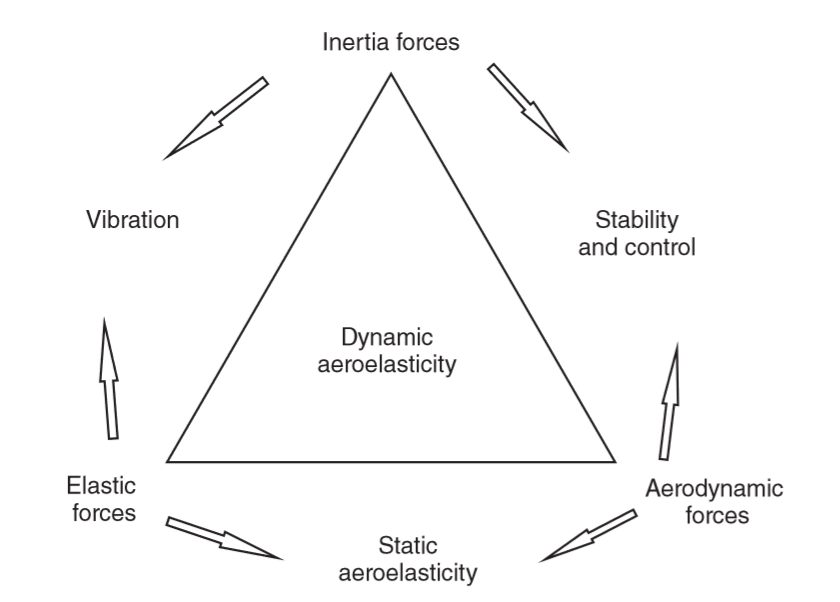
\includegraphics[width=8.5cm]{figures/aeroelas_triangle.png}
    \caption{Aeroelastic triangle}
    \label{fig:aero-tri}
\end{wrapfigure} 
%----------------------------------------

This study will investigate the affects of torsional stiffness and bending stiffness on the occurrence of flutter and divergence in a high AR wing. The study involves the three main forces that contribute to aeroelasticity: aerodynamic, elastic and inertia (as shown in figure \ref{fig:aero-tri}).\\

High AR wing are more flexible. This means elastic deformation is due to happen at large as the aircraft travels at higher speed. The need to understand aeroelastic phenomena in a high AR wing aircraft travelling near the transonic region was mentioned by Afonso et al \cite{Afonso2017AWings} for future development of high AR wing commercial jets.

\subsubsection{Inertia}
The inertia matrix can be represented as 
\begin{gather*}
    \begin{bmatrix}A_{bb} & A_{bt} \\ A_{tb} & A_{tt} \end{bmatrix}
\end{gather*}
However, as there is no inertia coupling in the model, $A_{bt} = A_{tb} = 0$ where $b$ represetns bending and $t$ represents torsion mode. This allows the bending stiffness ($EI$) and the torsional stiffness ($GJ$) to be represented in term of the torsion and bending natural frequencies as
\begin{equation}
    \omega_b = \sqrt{\frac{4EI}{A_{bb}s^3}} \text{ and } \omega_t = \sqrt{\frac{GJ}{A_{tt}s}}
\end{equation}

\subsubsection{Aerodynamics}
The aerodynamic model implemented here is a strip theory aerodynamics with additional simplified unsteady aerodynamic terms. This model includes the frequency dependent effect on lift and pitching moment which is essential for flutter analysis. The simplified expressions for lift increments ($dL$) and nose up pitching moment ($dM$) as a result of generalised unsteady aerodynamic forces applied with the strip theory are 
\begin{align}
dL &= \frac{1}{2}\rho V^2ca_w\Big( \frac{y^2\dot{q_1}}{s^2V}+\frac{y}{s}q_2\Big)dy\\
dM &= \frac{1}{2}\rho V^2 c^2\Big[ea_w\Big(\frac{y^2\dot{q_1}}{s^2V}+\frac{y}{s}q_2\Big)+M_{\dot{\theta}}c\frac{(y\dot{q_2})}{4sV}\Big]dy
%\label{eq:unsteady-aero-moment}
\end{align}
\iffalse
\begin{align}
L &= \rho V^2 \Big{(}L_z z + L_{\dot z}\frac{b\dot z}{V}+L_{\theta}b\theta + L_{\dot \theta}\frac{b^2 \dot \theta}{V}\Big{)} \\
M &= \rho V^2 \Big{(} M_z bz + M_{\dot z} \frac{b^2 \dot z}{V} + M_{\theta} b^2 \theta + M_{\dot \theta} \frac{b^3 \dot \theta}{V} \Big{)}
\end{align}
\fi

The change in lift due to a change in angle of incidence as modelled using an unsteady aerodynamic model can be illustrated by the Wagner Function (figure \ref{fig:wagner}). The function shows that lift takes time to build up as the  airflow travels across the semi-chord of the lifting surface. The quasi-steady model assumes a sharp step change in lift as it does not include time-effect; assumes instantaneous. This can results in a substantial aeroelastic modelling errors \cite{Wright2015INTRODUCTIONLOADS}. The pitch damping term $M_{\dot{\theta}}$ is included in equation (2) to include the time delay effect. This property is negative and will be treated as a constant in this 'simplified' model.

\begin{figure}[H]
    \centering
    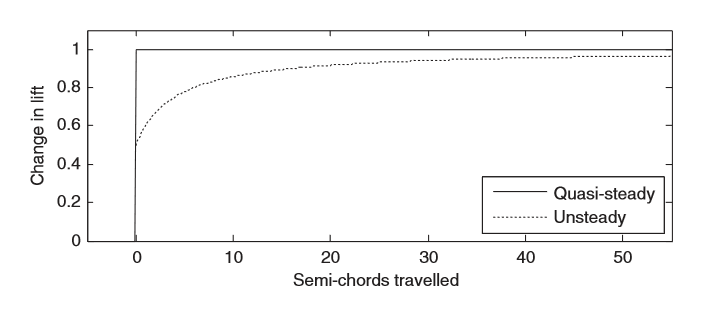
\includegraphics[width = .7\textwidth]{figures/wagner.png}
    \caption{Change in lift due to change in angle of incidence.}
    \label{fig:wagner}
\end{figure}


\subsubsection{Structure}
The structural model used in this analysis is the binary wing aeroelastic model. This implies that the wing is a flexible rectangular, unswept, cantilever wing with one bending and one torsion assumed shape (as shown in figure \ref{fig:free-free}).
\begin{figure}[H]
    \centering
    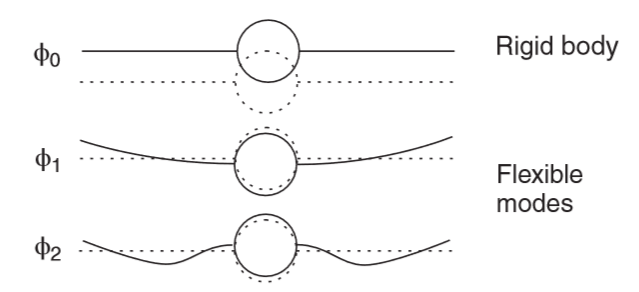
\includegraphics[width = .6\textwidth]{figures/free-free-mode-shape.png}
    \caption{Full aircraft 'Free-Free' assumed mode shapes}
    \label{fig:free-free}
\end{figure}
The kinetic energy due to the dynamic motion in bending and torsion can be written as
\begin{equation}
    T = \frac{m}{2}\int_0^s \int_0^c \Big( \Big{(} \frac{y}{s}\Big{)}^2\dot{q_1}+\Big{(}\frac{y}{s}\Big{)}(x-x_f)\dot{q_2}\Big{)}^2dxdy
\end{equation}
The elastic potential energy corresponds to the strain energy in bending and torsion can be represented as
\begin{equation}
    U = \frac{1}{2}\int_0^s EI \Big{(}\frac{2q_1}{s^2}\Big{)}^2dy+\frac{1}{2}\int_0^sGJ\Big{(}\frac{q_2}{s}\Big{)}^2dy
\end{equation}

Where $q_1$ and $q_2$ are generalised coordinates corresponding to the simple assumed shapes $\psi_1$ and $\psi_2$ as shown in figure \ref{fig:free-free}. Uniformed distribution of mass is assumed here. 


\subsection{Aeroelastic phenomena}
Aeroelastic phenomena can be categorised into two categories: dynamic and static.

\iffalse
\begin{figure}[H]
    \centering
    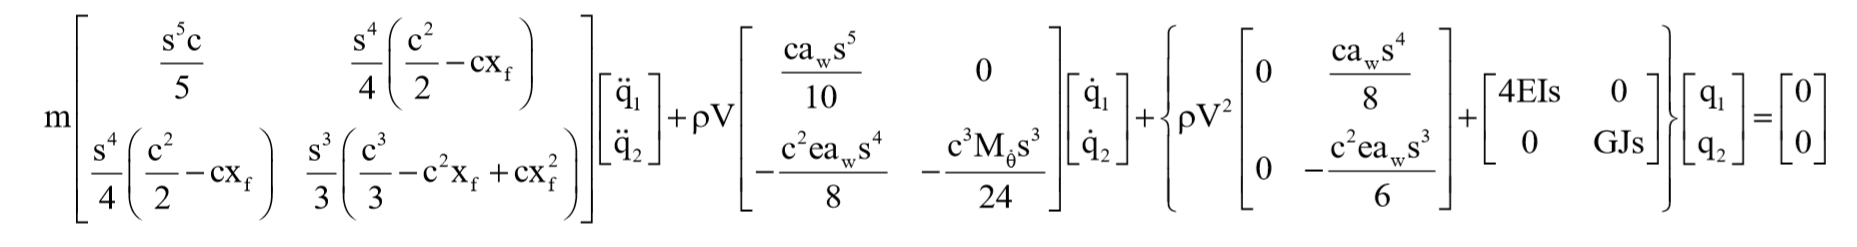
\includegraphics[width=\textwidth]{figures/EQ.png}
    %\caption{Full Aeroelastic Equation}
    \label{fig:aero-eq}
\end{figure}
\fi

\textbf{Apply Lagrange to get this}

\begin{gather}
\begin{split}
    m\begin{bmatrix} \frac{s^5c}{5} & \frac{s^4}{4}\Big{(}\frac{c^2}{2}-cx_f\Big{)} \\ \frac{s^4}{4}\Big{(}\frac{c^2}{2}-cx_f\Big{)} & \frac{s^3}{3}\Big{(}\frac{c^3}{3}-c^2x_f+cx_f^2\Big{)} \end{bmatrix} \begin{bmatrix}\ddot{q_1}\\ \ddot{q_2} \end{bmatrix} + \rho V \begin{bmatrix} \frac{ca_w s^5}{10} & 0 \\ -\frac{c^2e a_w s^4}{8} & -\frac{c^3M_{\dot\theta}s^3}{24} \end{bmatrix}\begin{bmatrix}\dot{q_1}\\ \dot{q_2}\end{bmatrix} +\\ \Bigg{\{}\rho V^2  \begin{bmatrix} 0 & \frac{ca_ws^4}{8} \\ 0 & -\frac{c^2ea_ws^3}{6} \end{bmatrix} + \begin{bmatrix} 4EIs & 0 \\ 0 & GJs \end{bmatrix} \Bigg{\}}\begin{bmatrix} q_1 \\ q_2 \end{bmatrix} = \begin{bmatrix} 0 \\ 0 \end{bmatrix}
\end{split}
\end{gather}

%Static  aeroelastic  phenomena involves  the  study  of  the  deformation  of  the  aircraft  and  how  this influences  the  distribution  of  lift.  This  con sequently  causes  torsional  divergence  reducing  the effectiveness of the control surface. Static aeroelasticity is also no affected by mass properties of the  aircraft  and  is  not  influenced  by  oscillations.  Dynamic  aeroelastic  phenomena  involves the analysis of  flutter of the  aircraft which disturbs the stability of the aircraft and the air stream is subjected to extraction of energy from the aircraft structure. 

\subsubsection{Flutter}
Flutter is the most important dynamic flutter phenomena \cite{MohammedFREEWINGS}. It occurs when an aircraft loses its stability due to an extraction of energy from the air stream by the aircraft structure. Resulting in an oscillatory motion that does not decay and increases in magnitude over time. This phenomenon is undesirable as it damages the aircraft structure and wear out its life cycle.\\

Flutter boundary is defined as  the lowest speed at which a small perturbation to a static equilibrium results in flutter. Lowest airspeed at which the system has a complex conjugate pair of eigenvalues with zero real part. 
\begin{figure}[h]
    \centering
    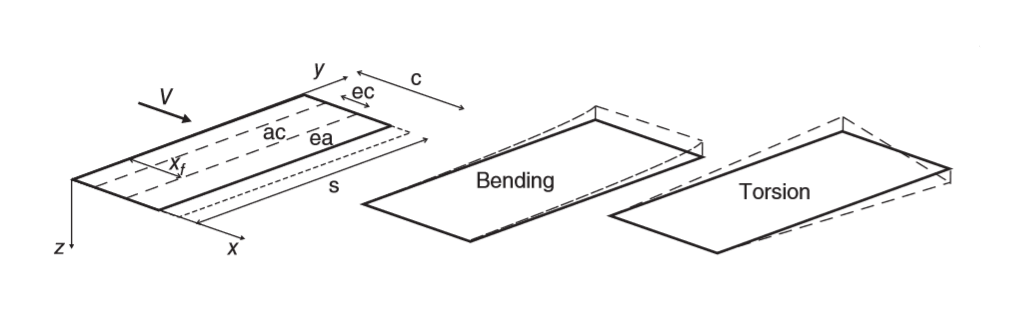
\includegraphics[width = .8\textwidth]{figures/torsion-bending-modes.png}
    \caption{Wing response to aerodynamic force in torsion and bending mode.}
    \label{fig:binary}
\end{figure}

\subsubsection{Divergence}
Divergence is a static instability of a lifting surface of an aircraft. When the wing exceeds its torsional divergence speed, the torsional moment from aerodynamic force due to twist overcomes the structural elastic restoring moment. This causes the wing to become statically unstable\cite{RaymondL.Bisplinghoff2002PrinciplesAeroelasticity}. As the time-dependent can be neglected in the case of static phenomena, the inertia force can be neglected. \\
%------ wrapped figure of heave and pitch -----
\begin{wrapfigure}{l}{8.5cm}
    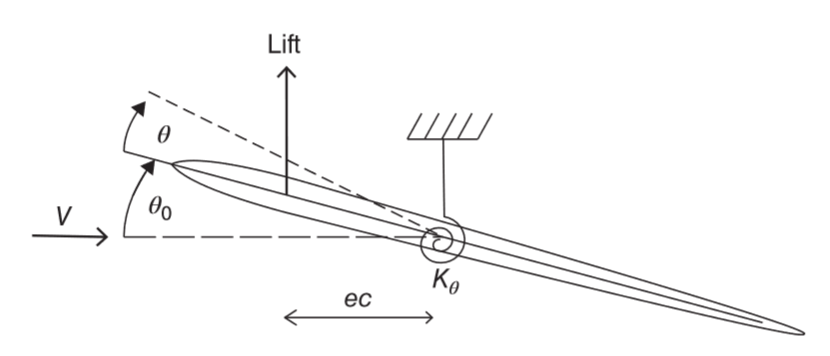
\includegraphics[width=8.5cm]{figures/two-dimensional-wing-torsional-spring.png}
    \caption{Two dimensional wing with a torsional spring.}
    \label{fig:torsional-spring}
\end{wrapfigure} 
%----------------------------------------
In a wing that is not stiff enough, divergence will cause the wing to twist off \cite{2011AeroelasticityFlutter}. Stiffness is much more important that strength in this case. In modern aircraft, flutter speed is usually lower than divergence speed; flutter usually occurs before divergence. However, this does not render divergence speed analysis to be obsolete as it is a good indication of the general stiffness of the aircraft structure and must be considered as part of the certification process \cite{Wright2015INTRODUCTIONLOADS}.\\ \\

Figure \ref{fig:torsional-spring} illustrates the torsional elastic moment($M_E$) versus the aerodynamic moment($M_{ac}$) and moment due to lift($ec.L$). Each term in the equilibrium can be expressed as:
\begin{eqnarray*}
ec.L = ec.qSC_{L,{\theta _0}}(\theta _0 + \theta),\hspace{1cm} M_{ac} = qScC_{M_{ac}},\hspace{1cm} M_E = K_{\theta}\theta
\end{eqnarray*}

%\begin{align*}
%\text{Lift:}\hspace{2cm} L &= qSC_{L,{\theta _0}}(\theta _0 + \theta)\\
%\text{Aero moment:}\hspace{1.6cm}M_{ac} &= qScC_{M_{ac}}\\
%\text{Elastic moment:}\hspace{1.65cm}M_E &= K_{\theta}\theta
%\end{align*}

\begin{equation}
qScC_{M_{ac}} + ec. qSC_{L,{\theta _0}}(\theta _0 + \theta) = K_{\theta}\theta
\end{equation}

\subsection{High AR Wing}

\begin{figure}[H]
    \centering
    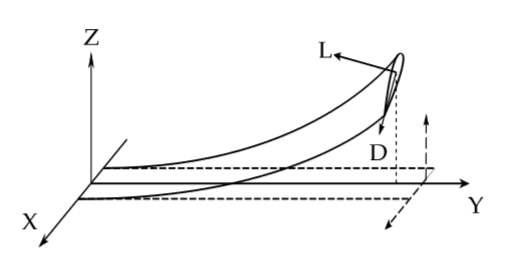
\includegraphics[width = .55\textwidth]{figures/Eaton-highly-flexible-wing.png}
    \caption{Nonlinear loading on a high AR wing.}
    \label{fig:high-AR-load}
\end{figure}


%%%%%%%%%%%%%%%%%%%%%%% LITERATURE REVIEW %%%%%%%%%%%%%%%%%%%%%%%
\subsection{Literature Review}
Afonso et al\cite{Afonso2017AWings} reviewed the importance of nonlinear model in aeroelasticity. The need for more computational and experimental study was mentioned as the existing reduced order model gets more complicte as nonlinearity inceases. The lack of information concerning values for modal amplitudes in simulations was also recognised.\\

In another study, Afonso et al \cite{Afonso2015LINEARWINGS} investigated the different analytical method using linear and nonlinear model. The differences between linear and nonlinear solutions grew more noticeable as the wing aspect-ratio increases. This was concluded to be a result of the reduction in wing mass, torsional stiffness and bending stiffness - the wing became more flexible. Afonso pointed out that a development of a nonlinear modelling to study the aeroelastic bahaviour is crucial for high-aspect-ratio wings.\\

Eaton et al \cite{EatonNumericalWings} explored a method that considered non-linearity, reduced-order beam model, linear quasi-steady strip theory aerodynamics and two-parameter bifurcation. This method was recommended for a study of limit-cycle-oscillations (LCO).\\
%The importance of the study of nonlinear aeroelasticity was also mentioned as more strives towards higher aspect ratio wing can be seen across the industry.\\

All of these studies established that nonlinear modelling is essential, Ritter, Teixeira and Cesnic's study compared different nonlinear aeroelastic methods for manoeuvre simulation of very flexible aircraft \cite{Ritter2018ComparisonAircraft}.\\

These studies mentioned above were focused on nonlinear study of the aeroelastic behaviour in high AR wings. However, the development of this model requires time and a better understanding of the field. It was decided that for the preliminary study at this lever, the linear model will be implemented and observed. The model developed in this project will be modified and improved into a nonlinear model in the Final Year Project.\\

The linear model used in this project was based on Jan R. Wright and Jonathan E. Cooper - Introduction to Aircraft Aeroelasticity and Loads \cite{Wright2015INTRODUCTIONLOADS}. 


%%%%%%%%%% Aim and Objectives %%%%%%%%%%
\section{Aim and Objectives - (1/2 page)}
\begin{itemize}
    \item Develop a computational method to study flutter and divergence behaviour.
    \item The aim is to use linear method for IXP to perform a preliminary parameter study.
    \item Develop into a nonlinear tool for FYP for a better study.
\end{itemize}

%%%%%%%%%% Technical/Scientific Methodology %%%%%%%%%%
\section{Methodology - (1-2 page)}
\begin{itemize}
    \item Computational and analytical method using eigenvalue solutions of the flutter equation.
    \item From existing code
    \item New one
    \item Different models
    \item Compare to existing experimental results
    \item Benchmarking against the existing results
    \item Use the code to analyse the aeroelastic behaviour of SUGAR High
\end{itemize}

%%%%%%%%%% Preliminary Studies %%%%%%%%%%
\section{Preliminary Studies - (3 page)}
\begin{figure}[H]
    \centering
    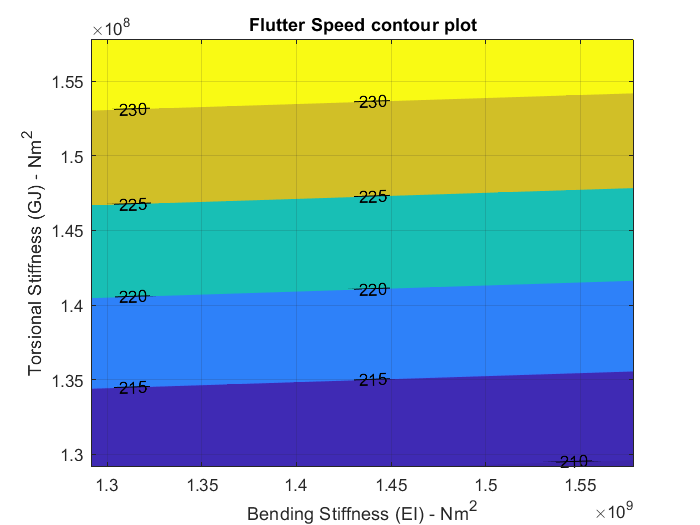
\includegraphics[width = .7\textwidth]{figures/SUGAR-High_flutter.png}
    \caption{Flutter speed plot for the SUGAR High conceptual wing}
    \label{fig:SUGAR-flutter}
\end{figure}

\begin{figure}[H]
    \centering
    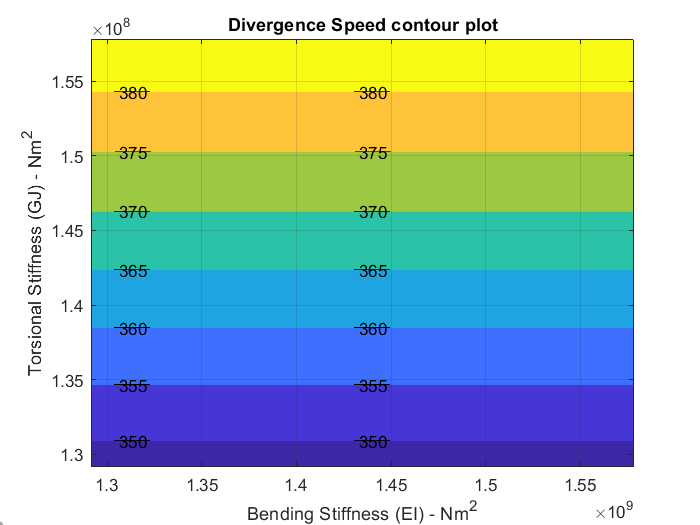
\includegraphics[width = .7\textwidth]{figures/SUGAR-High_divergence.png}
    \caption{Divergence speed plot for the SUGAR High conceptual wing}
    \label{fig:SUGAR-divergence}
\end{figure}

\subsection{Initial Conclusions - (1/2 page)}

%%%%%%%%%% Initial Conclusions and Risk Management %%%%%%%%%%
\section{Risk Management - (1/2 page)}

%%%%%%%%%% Future Work %%%%%%%%%%
\section{Future Work - (1/2 page)}
\begin{itemize}
    \item other parameters
    \item nonlinear
\end{itemize}

%%%%%%%%%% Project Work plan %%%%%%%%%%
\section{Work Plan}

%%%%%%%%%% Reference %%%%%%%%%%
\bibliography{references.bib}

%%%%%%%%%% Appendices %%%%%%%%%%
\section*{Appendix}

\end{document}
